\section{IR of Industrial Compilers}
\frame{
\frametitle{IR of Industrial Compilers :: LLVM Bitcode \\
How to generate IR for while statements?
}
\begin{columns}
\begin{column}{0.80\textwidth}
\begin{center}
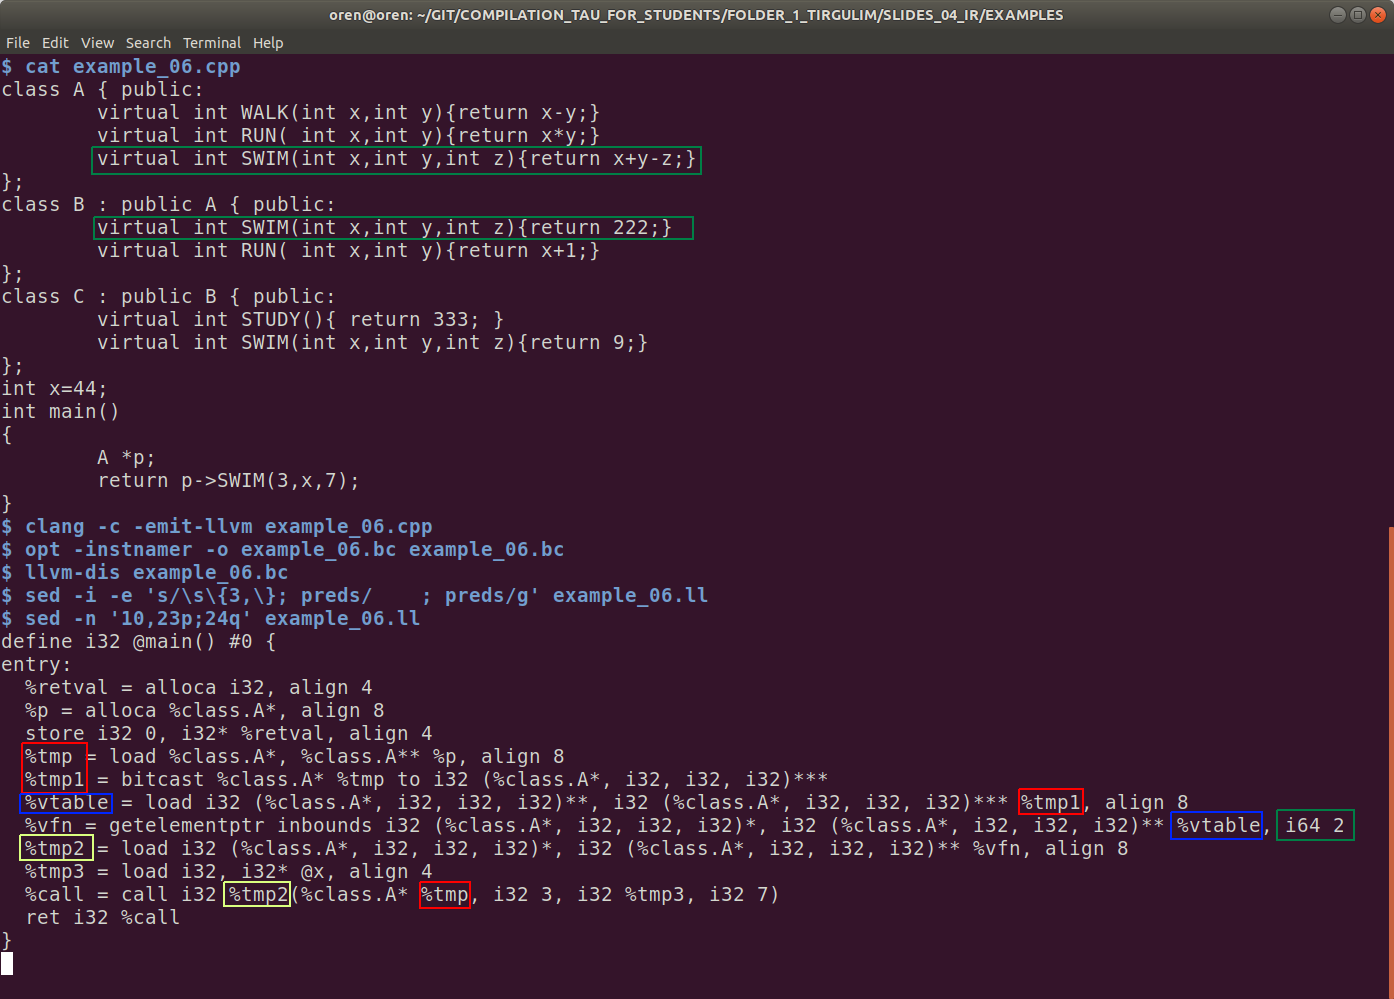
\includegraphics[width=0.95\textwidth]{example_06.png}
\end{center}
\end{column}
\begin{column}{0.4\textwidth}
\begin{itemize}
\item
load \textit{this} to {\color{red} tmp}
\item
load the virtual\\
function table  \\
to {\color{blue} vtable}
\item
use offset = {\color{green} 2}  \\
within {\color{blue} vtable}    \\
for method {\color{green} swim} \\
load it to {\color{yellow} tmp2}
\item
pass \textit{this} as the \\
first parameter           \\
to the method
\end{itemize}
\end{column}
\end{columns}
}